% Two clusters, Fiedler vector and sweep cut (generated by figs_c1ch09.py).
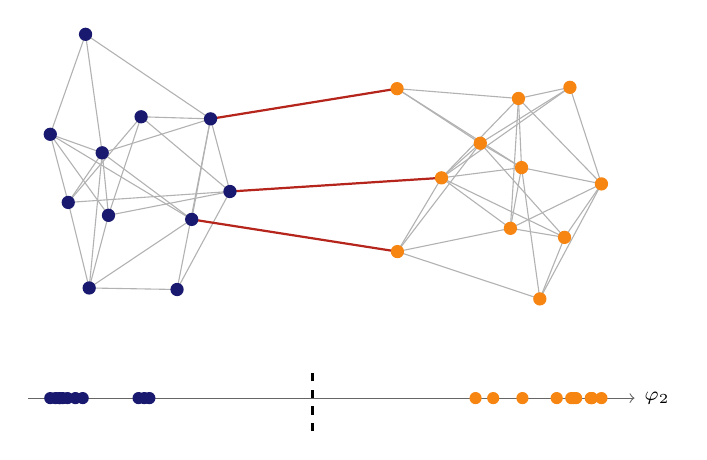
\begin{tikzpicture}[x=1.4cm,y=1.4cm]
\draw[black!30] (1.454,2.833) -- (1.150,1.285);
\draw[black!30] (1.454,2.833) -- (1.283,1.921);
\draw[black!30] (1.454,2.833) -- (0.824,2.852);
\draw[black!30] (1.454,2.833) -- (1.630,2.174);
\draw[black!30] (1.454,2.833) -- (0.471,2.525);
\draw[black!30] (1.454,2.833) -- (0.320,3.600);
\draw[BrickRed,thick] (1.454,2.833) -- (3.146,3.107);
\draw[black!30] (1.150,1.285) -- (0.353,1.299);
\draw[black!30] (1.150,1.285) -- (1.630,2.174);
\draw[black!30] (0.353,1.299) -- (1.283,1.921);
\draw[black!30] (0.353,1.299) -- (0.528,1.958);
\draw[black!30] (0.353,1.299) -- (0.163,2.075);
\draw[black!30] (0.353,1.299) -- (0.471,2.525);
\draw[black!30] (1.283,1.921) -- (0.000,2.693);
\draw[black!30] (1.283,1.921) -- (0.471,2.525);
\draw[BrickRed,thick] (1.283,1.921) -- (3.149,1.629);
\draw[black!30] (0.000,2.693) -- (0.528,1.958);
\draw[black!30] (0.000,2.693) -- (0.163,2.075);
\draw[black!30] (0.000,2.693) -- (0.471,2.525);
\draw[black!30] (0.000,2.693) -- (0.320,3.600);
\draw[black!30] (0.528,1.958) -- (0.824,2.852);
\draw[black!30] (0.528,1.958) -- (1.630,2.174);
\draw[black!30] (0.528,1.958) -- (0.471,2.525);
\draw[black!30] (0.824,2.852) -- (1.630,2.174);
\draw[black!30] (0.824,2.852) -- (0.163,2.075);
\draw[black!30] (1.630,2.174) -- (0.163,2.075);
\draw[BrickRed,thick] (1.630,2.174) -- (3.549,2.298);
\draw[black!30] (0.163,2.075) -- (0.471,2.525);
\draw[black!30] (0.471,2.525) -- (0.320,3.600);
\draw[black!30] (3.146,3.107) -- (3.901,2.612);
\draw[black!30] (3.146,3.107) -- (4.275,2.391);
\draw[black!30] (3.146,3.107) -- (4.247,3.018);
\draw[black!30] (3.901,2.612) -- (4.665,1.758);
\draw[black!30] (3.901,2.612) -- (3.149,1.629);
\draw[black!30] (3.901,2.612) -- (4.275,2.391);
\draw[black!30] (3.901,2.612) -- (3.549,2.298);
\draw[black!30] (3.901,2.612) -- (4.714,3.119);
\draw[black!30] (4.665,1.758) -- (5.000,2.243);
\draw[black!30] (4.665,1.758) -- (4.174,1.840);
\draw[black!30] (4.665,1.758) -- (4.441,1.200);
\draw[black!30] (4.665,1.758) -- (3.549,2.298);
\draw[black!30] (5.000,2.243) -- (4.174,1.840);
\draw[black!30] (5.000,2.243) -- (4.441,1.200);
\draw[black!30] (5.000,2.243) -- (4.275,2.391);
\draw[black!30] (5.000,2.243) -- (4.714,3.119);
\draw[black!30] (5.000,2.243) -- (4.247,3.018);
\draw[black!30] (4.174,1.840) -- (3.149,1.629);
\draw[black!30] (4.174,1.840) -- (4.275,2.391);
\draw[black!30] (4.174,1.840) -- (3.549,2.298);
\draw[black!30] (4.174,1.840) -- (4.247,3.018);
\draw[black!30] (3.149,1.629) -- (4.441,1.200);
\draw[black!30] (3.149,1.629) -- (3.549,2.298);
\draw[black!30] (4.441,1.200) -- (4.275,2.391);
\draw[black!30] (4.275,2.391) -- (3.549,2.298);
\draw[black!30] (4.275,2.391) -- (4.247,3.018);
\draw[black!30] (3.549,2.298) -- (4.714,3.119);
\draw[black!30] (3.549,2.298) -- (4.247,3.018);
\draw[black!30] (4.714,3.119) -- (4.247,3.018);
\fill[MidnightBlue] (1.454,2.833) circle (2.4pt);
\fill[MidnightBlue] (1.150,1.285) circle (2.4pt);
\fill[MidnightBlue] (0.353,1.299) circle (2.4pt);
\fill[MidnightBlue] (1.283,1.921) circle (2.4pt);
\fill[MidnightBlue] (0.000,2.693) circle (2.4pt);
\fill[MidnightBlue] (0.528,1.958) circle (2.4pt);
\fill[MidnightBlue] (0.824,2.852) circle (2.4pt);
\fill[MidnightBlue] (1.630,2.174) circle (2.4pt);
\fill[MidnightBlue] (0.163,2.075) circle (2.4pt);
\fill[MidnightBlue] (0.471,2.525) circle (2.4pt);
\fill[MidnightBlue] (0.320,3.600) circle (2.4pt);
\fill[BurntOrange] (3.146,3.107) circle (2.4pt);
\fill[BurntOrange] (3.901,2.612) circle (2.4pt);
\fill[BurntOrange] (4.665,1.758) circle (2.4pt);
\fill[BurntOrange] (5.000,2.243) circle (2.4pt);
\fill[BurntOrange] (4.174,1.840) circle (2.4pt);
\fill[BurntOrange] (3.149,1.629) circle (2.4pt);
\fill[BurntOrange] (4.441,1.200) circle (2.4pt);
\fill[BurntOrange] (4.275,2.391) circle (2.4pt);
\fill[BurntOrange] (3.549,2.298) circle (2.4pt);
\fill[BurntOrange] (4.714,3.119) circle (2.4pt);
\fill[BurntOrange] (4.247,3.018) circle (2.4pt);
\draw[->,black!60] (-0.2,0.3) -- (5.3,0.3);
\fill[MidnightBlue] (0.801,0.3) circle (2.2pt);
\fill[MidnightBlue] (0.294,0.3) circle (2.2pt);
\fill[MidnightBlue] (0.112,0.3) circle (2.2pt);
\fill[MidnightBlue] (0.899,0.3) circle (2.2pt);
\fill[MidnightBlue] (0.048,0.3) circle (2.2pt);
\fill[MidnightBlue] (0.085,0.3) circle (2.2pt);
\fill[MidnightBlue] (0.228,0.3) circle (2.2pt);
\fill[MidnightBlue] (0.853,0.3) circle (2.2pt);
\fill[MidnightBlue] (0.085,0.3) circle (2.2pt);
\fill[MidnightBlue] (0.156,0.3) circle (2.2pt);
\fill[MidnightBlue] (0.000,0.3) circle (2.2pt);
\fill[BurntOrange] (3.858,0.3) circle (2.2pt);
\fill[BurntOrange] (4.594,0.3) circle (2.2pt);
\fill[BurntOrange] (4.911,0.3) circle (2.2pt);
\fill[BurntOrange] (5.000,0.3) circle (2.2pt);
\fill[BurntOrange] (4.770,0.3) circle (2.2pt);
\fill[BurntOrange] (4.018,0.3) circle (2.2pt);
\fill[BurntOrange] (4.913,0.3) circle (2.2pt);
\fill[BurntOrange] (4.726,0.3) circle (2.2pt);
\fill[BurntOrange] (4.283,0.3) circle (2.2pt);
\fill[BurntOrange] (4.903,0.3) circle (2.2pt);
\fill[BurntOrange] (4.745,0.3) circle (2.2pt);
\draw[dashed,thick] (2.379,0.0) -- (2.379,0.6);
\node[font=\scriptsize,anchor=west] at (5.3,0.3) {$\varphi_2$};
\end{tikzpicture}
